\section{Experiments}
\label{sec:results}

We trained and evaluated \textbf{Deepseek-Distill-Llama3-8B} (Llama3-8B) \citep{grattafiori2024llama, guo2025deepseek} and \textbf{Qwen3-4B} \citep{yang2025qwen3technicalreport} in think mode on UnsolvableQA, reporting AVG@8 for AIME partitions and AVG@4 elsewhere. In our standardized setup, the final Qwen3-4B and Llama3-8B models are trained for 320 and 400 steps, respectively, while the ablation models were trained for 120 steps due to computational cost constraints.


\subsection{Main Results: Learning Solvability Boundaries}
\label{main_exp_}

\paragraph{UnsolvableRL significantly enhances reasoning reliability across architectures.} 
As shown in Table~\ref{tab:vertical_main_results_compact}, applying our framework to Llama3-8B improves its mean reasoning score from 25.2\% to \textbf{55.1\%}. Similarly, Qwen3-4B achieves a competitive global mean of \textbf{78.6\%}, substantially narrowing the gap with massive proprietary models such as GPT-5.2-Low and Gemini-3. Crucially, the 4B model achieves an unsolvable detection rate ($U$) of \textbf{87.5\%} while simultaneously boosting its solvable accuracy ($S$) from 43.4\% to \textbf{69.4\%}.\vspace{-2pt}

\paragraph{Performance gains generalize effectively to external OOD benchmarks.}
Beyond in-domain evaluations, aligned models show consistent improvements on MMLU-Pro, GPQA, and the externally-constructed unsolvable mathematics benchmark ReliableMath, as well as two distinct OOD logic tasks (8-Puzzle and Zebra Logic) detailed in \ref{sec:appendix_ood}. Notably, on \textbf{ReliableMath}, Llama3-8B achieves \textbf{68.3\%} (a +12.1pp gain), demonstrating strong competitiveness against much larger systems. Similarly, GPQA shows a \textbf{+12.0pp} increase in identifying graduate-level unsolvable instances. Detailed breakdowns are provided in Appendices~\ref{sec:appendix_comprehensive} \& \ref{sec:appendix_ood}. Beyond binary boundary learning, we further evaluate fine-grained defect attribution and zero-shot clarification transfer (\S\ref{sec:diagnostic_reasoning}).


\subsection{Fine-grained Diagnosis and Clarification Transfer}
\label{sec:diagnostic_reasoning}

To move beyond binary detection, we extend our framework into a Diagnostic Reasoning stage. In structured reasoning domains, we instantiate two answerability-defect families: Missing Information (MI) and Constraint Conflict (CC). MI denotes missing support needed for a determinate answer under the requested response format, while CC captures mutually incompatible observed constraints that make the problem specification inconsistent (AIME-CC uses the \texttt{unsolvable\_constraint\_contradiction} tag to operationalize this family).

To support this, we utilize seeds from AIME (1983) and the MMLU-Pro validation set to synthesize a diagnostic training set of 259 instances (120 solvable and 139 unsolvable), covering only missing-information and constraint-conflict families. For rigorous evaluation, we curate a separate diagnostic OOD test set comprising 320 instances from entirely disjoint sources: 149 diagnostic instances from AIME (2024--2025), distinct from the core AIME split in Table~\ref{tab:dataset_stats} and including additional MI cases for attribution evaluation, to evaluate temporal generalization; and 171 instances from GPQA (denoted as GPQA-U) to assess cross-domain transferability in graduate-level science. Models were initialized from converged UnsolvableRL checkpoints and underwent an additional 80-step diagnostic fine-tuning phase on the synthesized training set to output specific tags (e.g., \texttt{unsolvable\_missing\_information} and \texttt{unsolvable\_constraint\_contradiction}).


\begin{table}[t]
\centering
\small
\resizebox{\columnwidth}{!}{
\begin{tabular}{l cc cc}
\toprule
\multirow{2}{*}{Metrics / Datasets} & \multicolumn{2}{c}{Qwen3-4B} & \multicolumn{2}{c}{Llama3-8B} \\
\cmidrule(lr){2-3} \cmidrule(lr){4-5}
 & Instruct & + Diag. & Distill & + Diag. \\
\midrule
\multicolumn{5}{l}{\textit{Reasoning Accuracy (Solvable S $\uparrow$)}} \\
MMLU-Pro & 62.0 & 65.4 & 52.4 & 54.8 \\
GPQA     & 54.1 & 55.8 & 34.5 & 50.0 \\
AIME     & 67.9 & 69.6 & 35.0 & 48.8 \\
\midrule
\multicolumn{5}{l}{\textit{Unsolvability Detection (Unsolvable U $\uparrow$)}} \\
GPQA-U   & 21.7 & 33.8 & 21.5 & 36.6 \\
AIME-MI  & 23.4 & 41.4 & 38.3 & 38.8 \\
AIME-CC  & 45.2 & 69.6 & 45.2 & 75.6 \\
\midrule
\multicolumn{5}{l}{\textit{Interactive Transfer (IN3 Benchmark)}} \\
Detail Recovery & 60.5 & 66.5 & 47.8 & 60.7 \\
Intention Coverage & 34.7 & 39.7 & 20.4 & 23.0 \\
Avg. Rounds      & 4.24 & 4.58 & 3.10 & 4.16 \\
\bottomrule
\end{tabular}}
\caption{Results for diagnostic reasoning and clarification transfer. +Diag. models show performance synergies and superior zero-shot transfer to interactive tasks (IN3), enabling proactive questioning.}
\label{tab:diagnostic_results}
\end{table}

The transition to fine-grained diagnosis yields three critical insights:

1) General Reasoning Synergies: As shown in Table~\ref{tab:diagnostic_results}, learning to attribute unsolvability further sharpens the model's logical boundaries on solvable tasks. Notably, diagnostic tuning surged Llama3-8B's GPQA accuracy from 34.5\% to 50.0\% (+15.5pp). This suggests that identifying the root cause of unsolvability is functionally synergetic with valid reasoning.

2) Specific Diagnostic Gains: Models achieve high precision in causal attribution. Qwen3-4B nearly doubled its detection rate on AIME-MI (23.4\% $\rightarrow$ 41.4\%) and significantly improved on CC (45.2\% $\rightarrow$ 69.6\%). This demonstrates that unsolvability detection is not a monolithic template-matching task but a multi-faceted reasoning skill.

3) Transfer to Interactive Clarification: To address the concern that solvability boundaries might lead to over-refusal, we evaluate zero-shot transfer on the IN3 benchmark \cite{qian-etal-2024-tell} (naturalistic multi-turn dialogues). We find that the boundary awareness learned from math and logic successfully translates into proactive clarification behavior. For Llama3-8B, the ability to recognize queries with missing support for a determinate answer and recover missing user details in open-ended chat surged from 47.8\% to 60.7\%. This confirms that our alignment enables the model to act as a helpful assistant that asks follow-up questions when information is missing, rather than merely hallucinating a confident answer or providing a passive refusal.


\subsection{Ablation: Data--Penalty Interaction and Capability Collapse}
\begin{figure}[t]
    \centering
    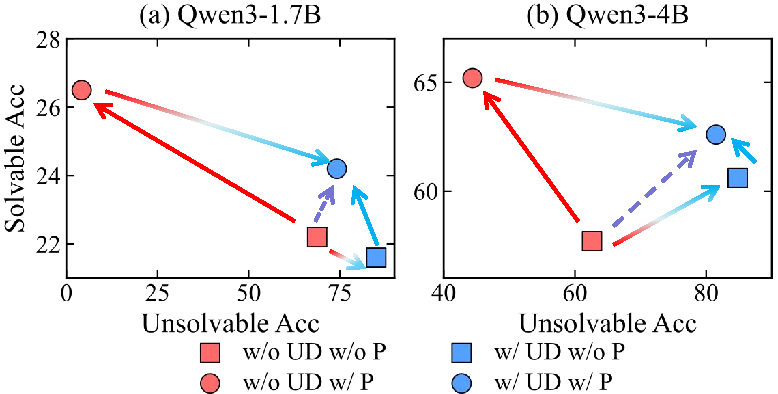
\includegraphics[width=\linewidth]{figures/s_and_u.pdf}
    \caption{Visualizing the interaction between Solvable Accuracy ($S$) and Unsolvable Detection ($U$). 
    The Purple Arrow highlights our full method (Blue Circle) achieving a Pareto improvement over the baseline (Red Square). 
    Both models exhibit consistent dynamics: applying penalties without Unsolvable Data (UD) triggers \textbf{Capability Collapse} (Red Arrow), sacrificing $U$ to maximize $S$. 
    Conversely, when paired with UD, the penalty acts as a \textbf{Regularizer} (Blue Arrow), trading marginal $U$ for significant gains in $S$ compared to using UD alone (Blue Square).
    }
    \label{fig:ablation_scatter}
\end{figure}
\begin{figure*}[t]
    \centering
    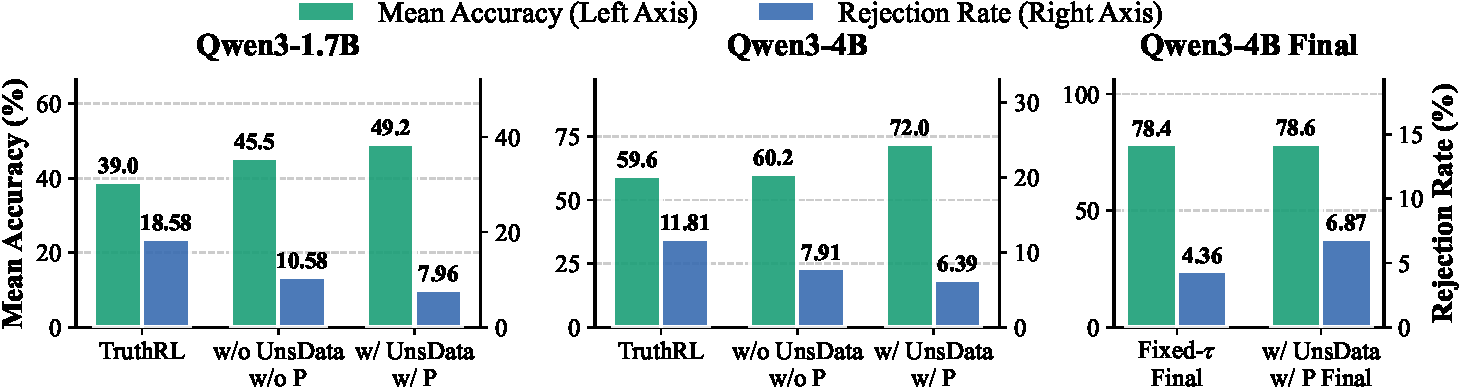
\includegraphics[width=1.0\linewidth]{figures/0105rej_rate_comparison.pdf}
    \caption{
        Performance Comparison and Calibration Analysis. 
        (Left/Middle) Comparison with TruthRL. While TruthRL achieves higher rejection rates (Blue bars), it suffers from over-refusal, significantly degrading Accuracy (Green bars).
        (Right) Comparison of threshold strategies. The adaptive mechanism (\textit{w/ P Final}) maintains a healthier rejection rate (6.87\%) compared to the Fixed-$\tau$ baseline (4.36\%) while preserving high accuracy.
    }
    \label{fig:performance_comparison}
\end{figure*}
To understand the contributions of data and reward mechanisms, we conducted a comprehensive ablation study comparing four configurations, defined by the inclusion of \textbf{Unsolvable Data (UnsData)} and the \textbf{False Unsolvability Penalty (P)}. Figure~\ref{fig:ablation_scatter} compares: (1) \textbf{w/o UnsData w/o P} (baseline); (2) \textbf{w/o UnsData w/ P} (penalty only); (3) \textbf{w/ UnsData w/o P} (data only); and (4) \textbf{w/ UnsData w/ P} (our full method). \vspace{-2pt}

\paragraph{Explicit Unsolvable Data is a Prerequisite for Detection.}
As shown in Figure~\ref{fig:ablation_scatter}, the naive baseline trained without unsolvable data (\textit{w/o UnsData}) lacks the fundamental capability to recognize unsolvability. For Qwen3-4B, detection is weak ($U=62.6\%$). Introducing explicit unsolvable data provides the necessary supervision, boosting detection significantly ($U \to 84.8\%$). This confirms that optimizing solely for reasoning correctness on solvable tasks is insufficient.\vspace{-5pt}

\paragraph{Applying Penalty without Data Triggers Capability Collapse.}
Figure~\ref{fig:ablation_scatter} (left) illustrates a critical failure mode caused by objective mismatch. When the penalty is enforced without providing ground-truth unsolvable examples, the model, lacking positive examples of valid refusal, minimizes the penalty risk by defaulting to answering all queries. This behavior effectively collapses its refusal mechanism, as seen in the 1.7B model's detection rate plummeting from 68.8\% to 4.2\%.\vspace{-5pt}

\paragraph{Applying Penalty with Data Facilitates a Strategic Trade-off.}
When grounded with adequate data, the penalty shifts from being a suppressor to a regularizer. For Qwen3-4B, adding the penalty (\textit{w/ UnsData w/ P}) improves Solvable Accuracy ($S$) from 60.6\% to 62.6\%, at the cost of a slight drop in detection ($U: 84.8\% \to 81.5\%$). This trade-off is strategic: it sacrifices marginal detection performance to enforce stricter reasoning rigor on feasible problems, optimizing the model for real-world utility.\vspace{-5pt}

\paragraph{Overall Gain: A Pareto Improvement over the Baseline.}
Viewing the trajectory globally (the purple dashed arrow in Figure~\ref{fig:ablation_scatter}b), our full method represents a comprehensive upgrade over the naive baseline (\textit{w/o UnsData w/o P}). We achieve significant gains in both dimensions for Qwen3-4B ($S: 57.7\% \to 62.6\%$, $U: 62.6\% \to 81.5\%$). This confirms that UnsolvableRL does not merely shift the decision boundary, but fundamentally enhances both reliability and reasoning capability.


\subsection{Calibration: Decoupling Objective Detection from Subjective Refusal}

\paragraph{Necessity of Decoupling Objective and Subjective Refusal.} 
We first investigated the necessity of decoupling objective detection from subjective calibration by training a baseline variant that conflates the two behaviors (i.e., the model outputs a unified \texttt{unsolvable} tag for any refusal, regardless of whether it stems from logical contradictions or subjective difficulty). We found that this undifferentiated approach results in significantly lower accuracy on solvable tasks across architectures. Specifically, after 120 training steps, the conflated model achieved a solvable set accuracy ($S$) of only 53.7\% for Qwen3-4B and a mere 14.9\% for Llama3-8B, compared to 62.6\% and 40.1\% achieved by our decoupled method at the same stage, respectively. This substantial performance gap, particularly evident in the Llama model, validates that distinguishing between ``the problem is logically flawed'' and ``the problem exceeds my current capacity'' is essential for preserving reasoning rigor; without this distinction, models tend to adopt a ``lazy'' refusal strategy to maximize rewards, severely discouraging attempts at complex reasoning. \textbf{Detailed training settings and a diagnostic analysis of this baseline are provided in Appendix~\ref{sec:mix_tag_analysis}.} \vspace{-5pt}


\paragraph{Superior Balance Compared to TruthRL.} We further benchmark our method against TruthRL~\citep{wei2025truthrl} and different thresholding strategies. 
As shown in Left/Middle panels of Figure~\ref{fig:performance_comparison}, TruthRL tends to be overly conservative, leading to over-refusal. For Qwen3-1.7B, while TruthRL achieves a high Rejection Rate (18.58\%), its Accuracy drops to 39.0\%, which is inferior to even the baseline. In contrast, our method achieves a significantly higher Accuracy (45.5\%) with a moderate and precise Rejection Rate (10.58\%). This indicates that our \textit{target accuracy threshold} provides a softer, more distinctive signal than TruthRL's hard refusal reward, preserving the model's core reasoning capabilities.\vspace{-5pt}

\paragraph{Dynamic Thresholding Prevents Overconfidence.}
The rightmost panel of Figure~\ref{fig:performance_comparison} highlights the importance of our dynamic calibration. The Fixed-$\tau$ baseline yields a low rejection rate (4.36\%), suggesting overconfidence. By dynamically adjusting $\tau$ based on the moving average of solvable confidence, our method (w/ P Final) maintains a robust rejection rate (6.87\%) without sacrificing accuracy (78.6\%), ensuring the model remains prudent even as it becomes stronger.
